%%%%%%%%%%%%%%%%%%%%%%%%%%%%%%%%%%%%
% Lesson Plan (50 minutes)
%%%%%%%%%%%%%%%%%%%%%%%%%%%%%%%%%%%%
\begin{frame}
    \frametitle{Lesson Plan}
    \begin{itemize}
        \item xx min Lecture: review residuals, correlation from last time
        \item xx min Lecture: how to "find" the best-fit line? different objectives - motivate least squares (like slide 12)
        \item xx min Lecture: conditions for least squares (linearity, nearly-normal residuals, constant variability)
        \item xx min R Demonstration: for an example problem, determine whether the conditions for least squares have been met 
        \item xx min Edfinity quiz: new examples, are the conditions met?
        \item xx min Lecture: slope and intercept, and their interpretations in regression 
        \item xx min R Demonstration: slope and intercept in the lecture example (from scratch, and using lm)
        \item xx min Edfinity quiz: practice interpreting the slope and intercept in new examples
        \item xx min R Demonstration: now that we have the slope and intercept, we can plot a regression line and make predictions
        \item xx min R Demonstration: extrapolation
        \item (if time) xx min Lecture: $R^2$ and its interpretation (can continue later)
    \end{itemize}
\end{frame}

%%%%%%%%%%%%%%%%%%%%%%%%%%%%%%%%%%%%
% Learning objectives:
%%%%%%%%%%%%%%%%%%%%%%%%%%%%%%%%%%%%
\begin{frame}
    \frametitle{Learning Objectives}
    \begin{itemize}
        \item \textbf{M1, LO1: Classify and Analyze Variables:} Categorize variables based on their types (e.g., numerical/categorical, continuous/discrete, ordinal), assess their association (positive, negative, or independent), and determine which make sense as explanatory vs. response variables.
        \item \textbf{M1, LO3: Use R for Data Management and Exploration:} Utilize R to load, pre-process, and explore data through visualization and summarization techniques.
        \item \textbf{M1, LO4: Visualize and Describe Data Distributions:} Select appropriate visualizations (scatterplots, histograms, box plots, bar plots) to depict data, and describe distributions qualitatively (shape, center, spread, outliers) and quantitatively (mean, median, mode, range, IQR, standard deviation).
        \item \textbf{M5, LO1: Describe and Assess Relationships Between Two Variables:} Describe the association between two numerical variables in a scatter plot in terms of direction, shape (linear or nonlinear), and strength, and assess whether linear regression is an appropriate model.    
        \item \textbf{M5, LO2: Compute and Interpret Correlation and R²:} Compute and interpret correlation coefficients and R² values, while recognizing that correlation does not imply causation. 
        \item \textbf{M5, LO3: Fit and Interpret Linear Models Using Least Squares:} Fit the intercept and slope of a linear model to data using the least squares method, interpret the fitted values, and use the model to predict responses to new inputs.
    \end{itemize}
\end{frame}
    
%%%%%%%%%%%%%%%%%%%%%%%%%%%%%%%%%%%%
% TODO: Copy and adapt these slides base on the lesson plan
%%%%%%%%%%%%%%%%%%%%%%%%%%%%%%%%%%%%

\section{Fitting a line by least squares regression}

%%%%%%%%%%%%%%%%%%%%%%%%%%%%%%%%%%%%

\subsection{Eyeballing the line}

%%%%%%%%%%%%%%%%%%%%%%%%%%%%%%%%%%%

\begin{frame}
\frametitle{Eyeballing the line}

\twocol{0.3}{0.7}
{
\pq{Which of the following appears to be the line that best fits the linear relationship between \% in poverty and \% HS grad? Choose one.}
\soln{\only<2>{\orange{
(a)
}}}
}
{
\begin{center}
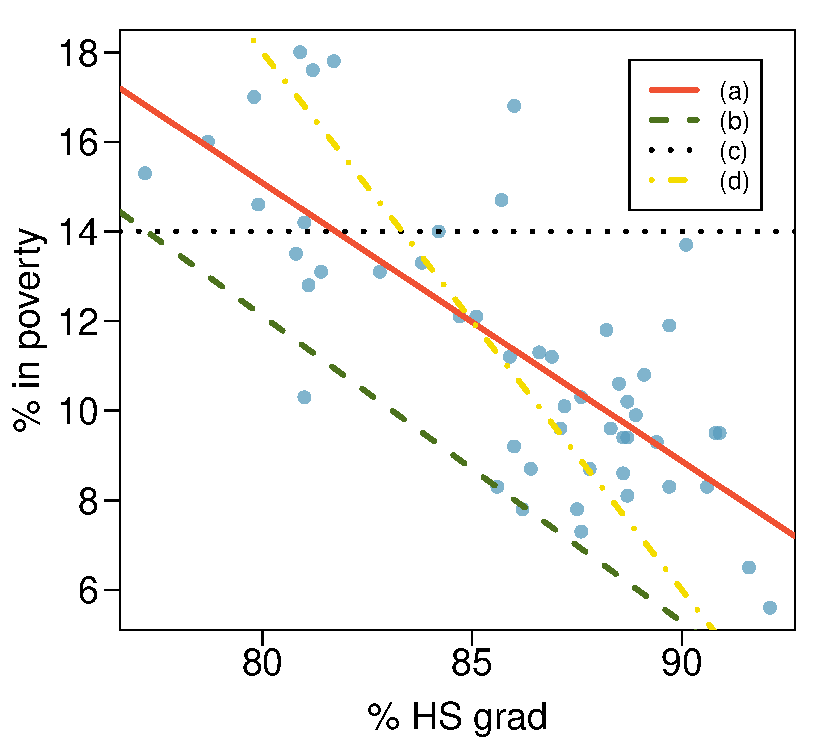
\includegraphics[width=\textwidth]{8-2_least_square_reg/figures/poverty/poverty_hsgrad_manylines}
\end{center}
}
\end{frame}

%%%%%%%%%%%%%%%%%%%%%%%%%%%%%%%%%%%

\subsection{Residuals}

%%%%%%%%%%%%%%%%%%%%%%%%%%%%%%%%%%%

\begin{frame}
\frametitle{Residuals}

\hl{Residuals} are the leftovers from the model fit: Data = Fit + Residual

\begin{center}
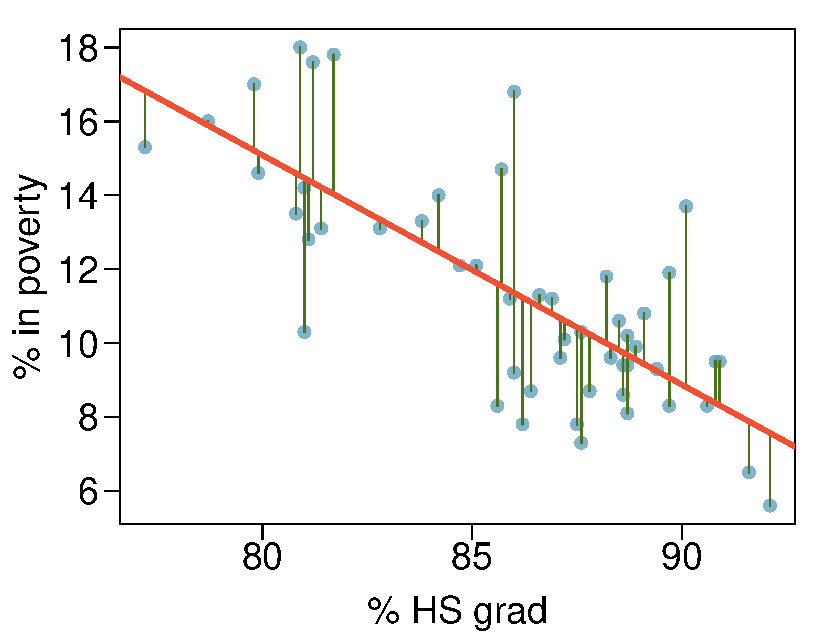
\includegraphics[width=0.8\textwidth]{8-2_least_square_reg/figures/poverty/poverty_hsgrad_res}
\end{center}

\end{frame}

%%%%%%%%%%%%%%%%%%%%%%%%%%%%%%%%%%

\begin{frame}
\frametitle{Residuals (cont.)}

\formula{Residual}{
Residual is the difference between the observed ($y_i$) and predicted $\hat{y}_i$. 
\[ e_i = y_i - \hat{y}_i \]
}
\vspace{-0.5cm}
\twocol{0.6}{0.4}
{
\begin{center}
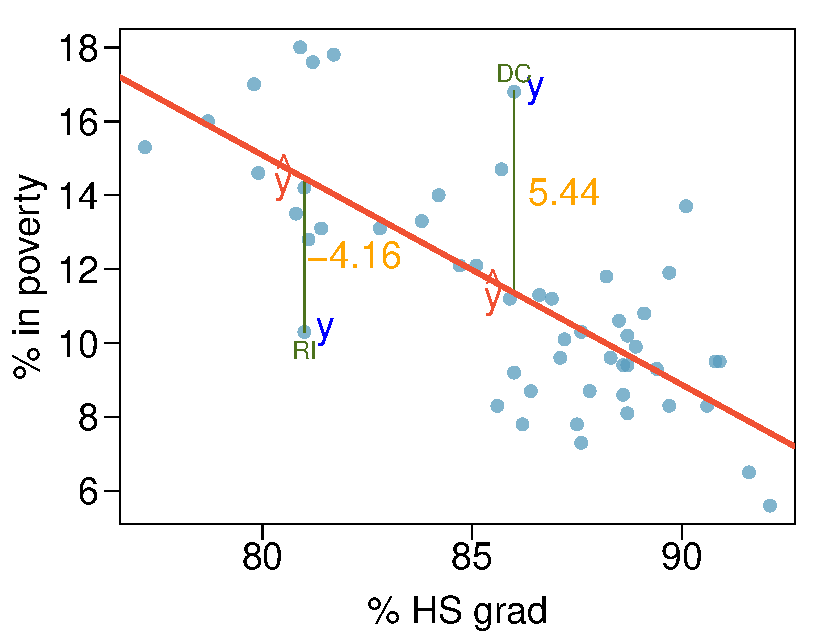
\includegraphics[width=\textwidth]{8-2_least_square_reg/figures/poverty/poverty_hsgrad_res_text}
\end{center}
}
{
\pause
\begin{itemize}
\item \% living in poverty in DC is 5.44\% more than predicted.
\pause
\item \% living in poverty in RI is 4.16\% less than predicted.
\end{itemize}
}


\end{frame}

%%%%%%%%%%%%%%%%%%%%%%%%%%%%%%%%%%

\subsection{Best line}

%%%%%%%%%%%%%%%%%%%%%%%%%%%%%%%%%%%

\begin{frame}
\frametitle{A measure for the best line}

\begin{itemize}

\item We want a line that has small residuals:
\pause
\begin{enumerate}
\item Option 1: Minimize the sum of magnitudes (absolute values) of residuals
\[ |e_1| + |e_2| + \cdots + |e_n| \]
\pause
\item Option 2: Minimize the sum of squared residuals -- \hl{least squares}
\[ e_1^2 + e_2^2 + \cdots + e_n^2 \]
\end{enumerate}

\pause

\item Why least squares?
\pause
\begin{enumerate}
\item Most commonly used
\pause
\item Easier to compute by hand and using software
\pause
\item In many applications, a residual twice as large as another is usually more than twice as bad
\end{enumerate}

\end{itemize}

\end{frame}

%%%%%%%%%%%%%%%%%%%%%%%%%%%%%%%%%%

\begin{frame}
\frametitle{The least squares line}

\[ \mathhl{ \hat{y} = \beta_0 + \beta_1 x } \]

\setlength{\unitlength}{0.75mm}
\begin{picture}(5,0)
\put(62.5,5){\vector(-2,-1){20}}
\put(18,-5){\orange{predicted y}}
\end{picture}

\begin{picture}(5,0)
\put(70,10){\vector(-1,-1){15}}
\put(50,-10){\orange{intercept}}
\end{picture}

\begin{picture}(5,0)
\put(80,15){\vector(1,-1){10}}
\put(90,0){\orange{slope}}
\end{picture}

\begin{picture}(5,0)
\put(90,22.5){\vector(2,-1){20}}
\put(110,8){\orange{explanatory variable}}
\end{picture}

\hl{Notation:}
\begin{itemize}

\item Intercept:
\begin{itemize}
\item Parameter: $\beta_0$ \\
\item Point estimate: $b_0$ \\
\end{itemize}

\item Slope:
\begin{itemize}
\item Parameter: $\beta_1$ \\
\item Point estimate: $b_1$ \\
\end{itemize}

\end{itemize}


\end{frame}

%%%%%%%%%%%%%%%%%%%%%%%%%%%%%%%%%%

\subsection{The least squares line}

%%%%%%%%%%%%%%%%%%%%%%%%%%%%%%%%%%%

\begin{frame}
\frametitle{Given...}

\twocol{0.5}{0.5}
{
\begin{center}
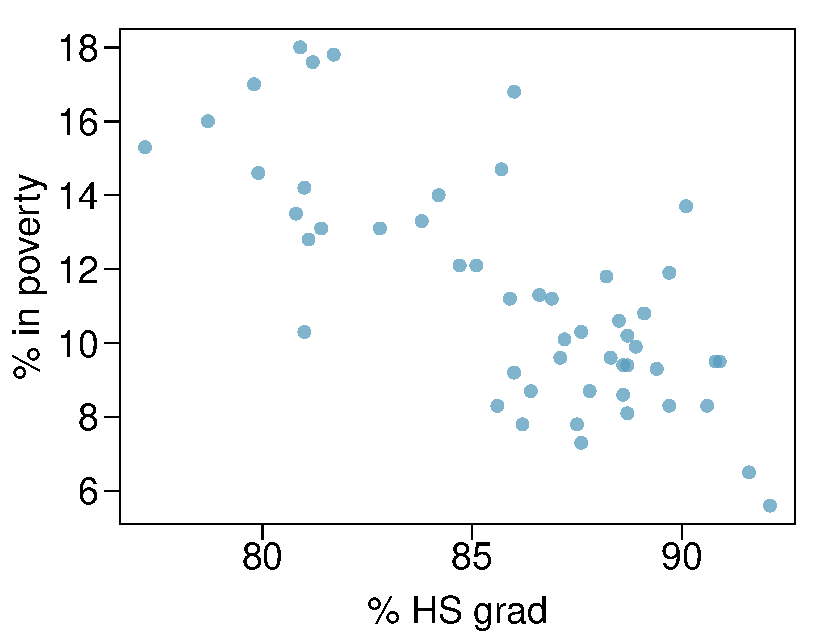
\includegraphics[width=\textwidth]{8-2_least_square_reg/figures/poverty/poverty_hsgrad}
\end{center}
}
{
\begin{tabular}{l r r}
\hline
		& \% HS grad		& \% in poverty \\
		& $(x)$			& $(y)$ \\
\hline
mean	& $\bar{x} = 86.01$	& $\bar{y} = 11.35$  \\
sd		& $s_x = 3.73$		& $s_y = 3.1$ \\
\hline
		& correlation		& $R = -0.75$ \\
\hline
\end{tabular}
}

\end{frame}

%%%%%%%%%%%%%%%%%%%%%%%%%%%%%%%%%%

\begin{frame}
\frametitle{Slope}

\formula{Slope}
{The slope of the regression can be calculated as 
\[ b_1 = \frac{s_y}{s_x} R \]
}

\pause

\hl{In context...}
\[ b_1 = \frac{3.1}{3.73} \times -0.75 = -0.62 \]

\pause
$\:$ \\
\hl{Interpretation} \\
For each additional \% point in HS graduate rate, we would expect the \% living in poverty to be lower on average by 0.62\% points.

\end{frame}

%%%%%%%%%%%%%%%%%%%%%%%%%%%%%%%%%%

\begin{frame}
\frametitle{Intercept}

\formula{Intercept}
{The intercept is where the regression line intersects the $y$-axis. The calculation of the intercept uses the fact the a regression line always passes through $(\bar{x},\bar{y})$.
\[ b_0 = \bar{y} - b_1 \bar{x} \]
}

\pause

\twocol{0.68}{0.32}
{
\begin{center}
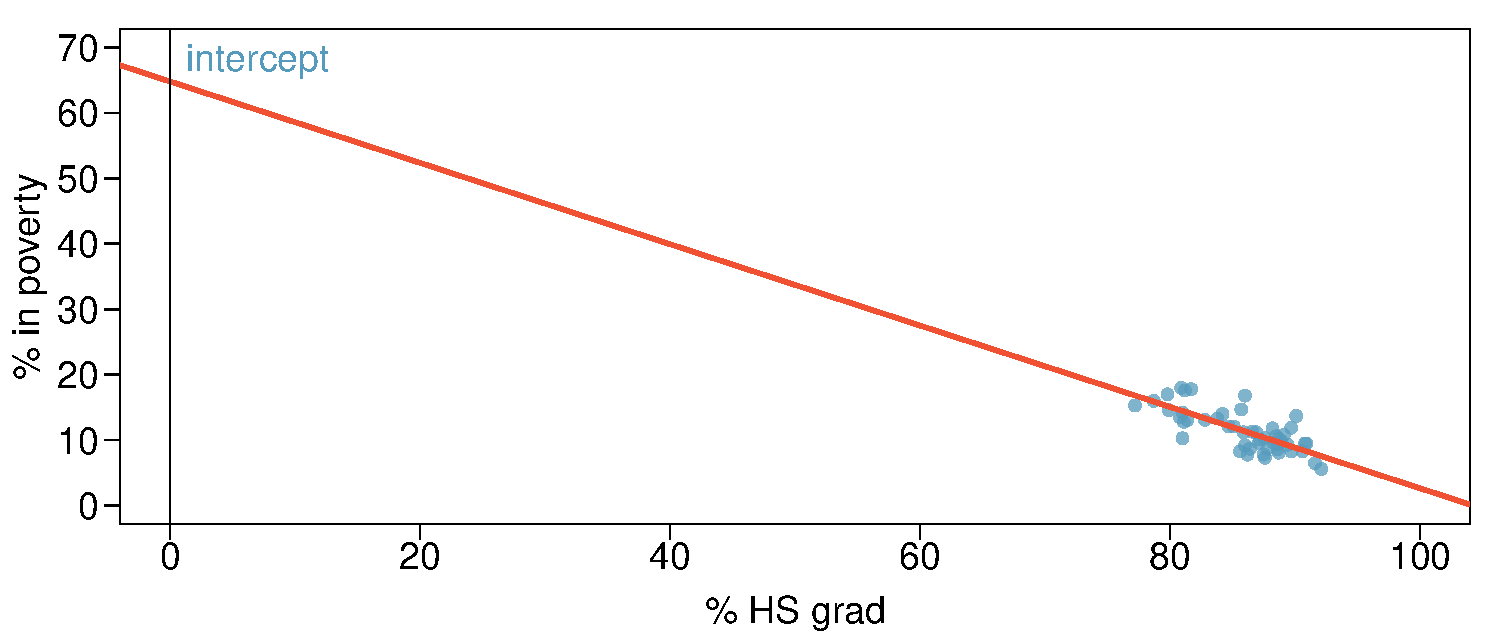
\includegraphics[width=\textwidth]{8-2_least_square_reg/figures/poverty/poverty_hsgrad_line_wide}
\end{center}
}
{
\pause
\begin{align*}
b_0 &= 11.35 - (-0.62) \times 86.01 \\
&= 64.68
\end{align*}
}

\end{frame}

%%%%%%%%%%%%%%%%%%%%%%%%%%%%%%%%%%

\begin{frame}
\frametitle{}

\pq{Which of the following is the correct interpretation of the intercept?}

\begin{enumerate}[(a)]
\item For each \% point increase in HS graduate rate, \% living in poverty is expected to increase on average by 64.68\%.
\item For each \% point decrease in HS graduate rate, \% living in poverty is expected to increase on average by 64.68\%.
\item Having no HS graduates leads to 64.68\% of residents living below the poverty line.
\solnMult{States with no HS graduates are expected on average to have 64.68\% of residents living below the poverty line.}
\item In states with no HS graduates \% living in poverty is expected to increase on average by 64.68\%.
\end{enumerate}

\end{frame}

%%%%%%%%%%%%%%%%%%%%%%%%%%%%%%%%%%%

\begin{frame}
\frametitle{More on the intercept}

Since there are no states in the dataset with no HS graduates, the intercept is of no interest, not very useful, and also not reliable since the predicted value of the intercept is so far from the bulk of the data.

\begin{center}
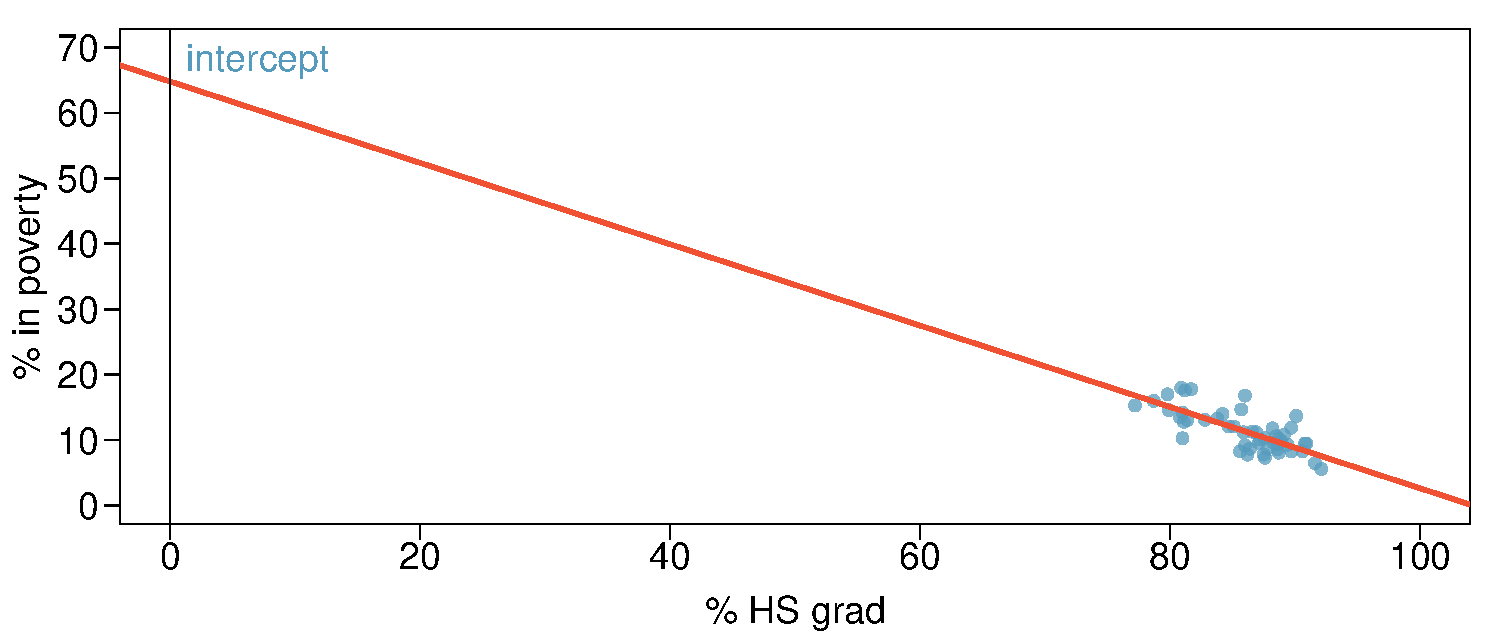
\includegraphics[width=\textwidth]{8-2_least_square_reg/figures/poverty/poverty_hsgrad_line_wide}
\end{center}

\end{frame}

%%%%%%%%%%%%%%%%%%%%%%%%%%%%%%%%%%

\begin{frame}
\frametitle{Regression line}

\[ \widehat{\%~in~poverty} = 64.68 - 0.62~\%~HS~grad \]

\begin{center}
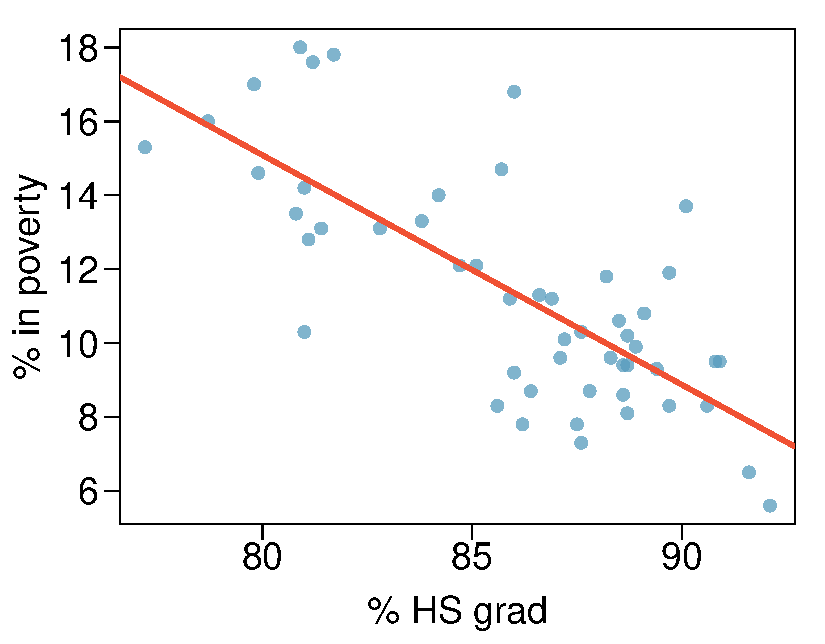
\includegraphics[width=0.7\textwidth]{8-2_least_square_reg/figures/poverty/poverty_hsgrad_line}
\end{center}

\end{frame}

%%%%%%%%%%%%%%%%%%%%%%%%%%%%%%%%%%

\subsection{Recap: Interpreting the slope and the intercept}

%%%%%%%%%%%%%%%%%%%%%%%%%%%%%%%%%%%

\begin{frame}
\frametitle{Interpretation of slope and intercept}

\twocol{0.5}{0.5}{
\begin{itemize}

\item \hl{Intercept:} When {$x = 0$}, {$y$} is expected to equal {the intercept}. \\

$\:$ \\

\item \hl{Slope:} For each {unit} in {$x$}, {$y$} is expected to {increase / decrease} on average by {the slope}.

\end{itemize}
}
{
\begin{center}
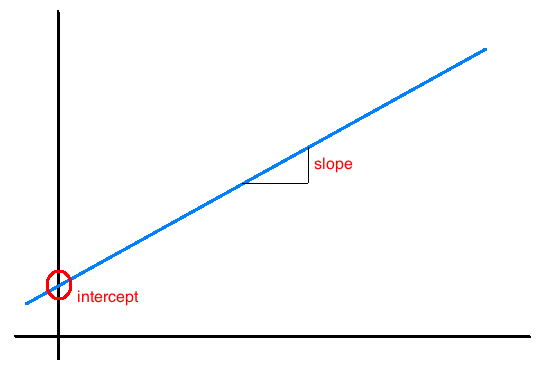
\includegraphics[width=\textwidth]{8-2_least_square_reg/figures/diagram}
\end{center}
}

\vspace{1cm}

\Note{These statements are not causal, unless the study is a randomized controlled experiment.}

\end{frame}


%%%%%%%%%%%%%%%%%%%%%%%%%%%%%%%%%%

\subsection{Prediction \& extrapolation}

%%%%%%%%%%%%%%%%%%%%%%%%%%%%%%%%%%


\begin{frame}
\frametitle{Prediction}

\begin{itemize}

\item Using the linear model to predict the value of the response variable for a given value of the explanatory variable is called \hl{prediction}, simply by plugging in the value of $x$ in the linear model equation.

\item There will be some uncertainty associated with the predicted value.

\end{itemize}

\begin{center}
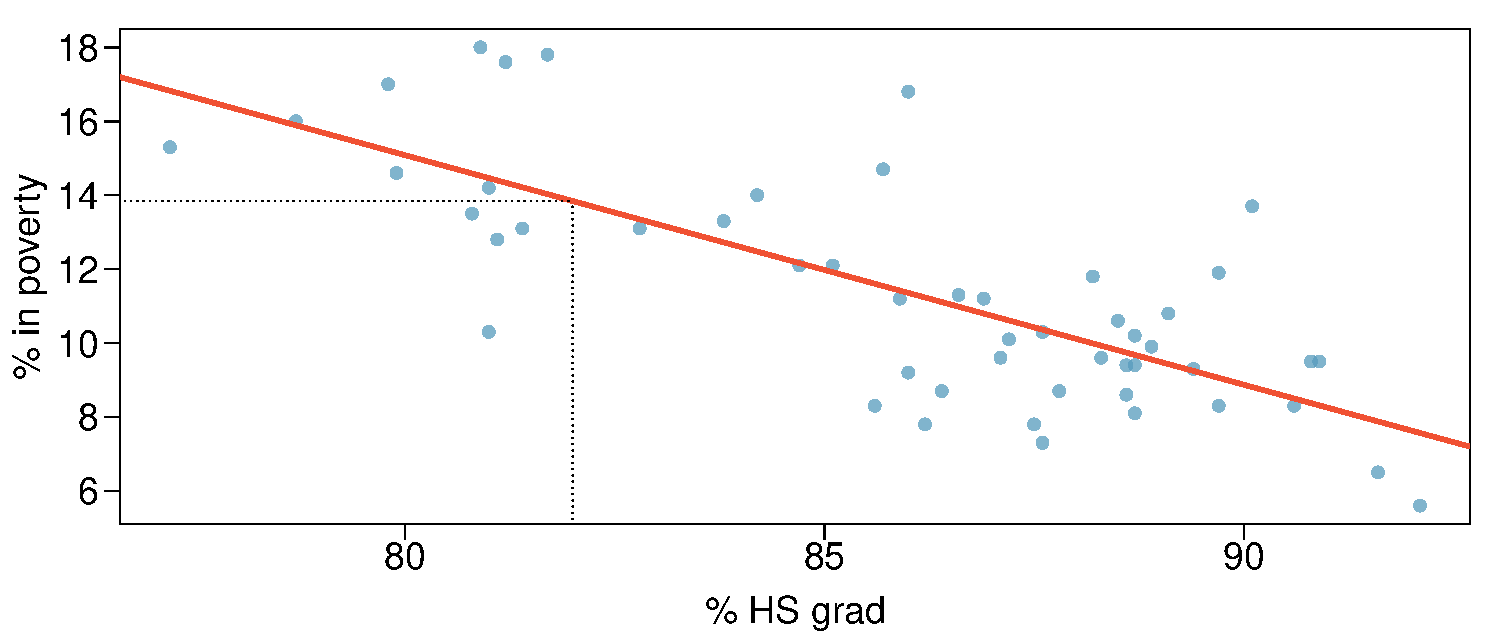
\includegraphics[width=0.9\textwidth]{8-2_least_square_reg/figures/poverty/poverty_hsgrad_pred}
\end{center}

\end{frame}

%%%%%%%%%%%%%%%%%%%%%%%%%%%%%%%%%%

\begin{frame}
\frametitle{Extrapolation}

\begin{itemize}

\item Applying a model estimate to values outside of the realm of the original data is called \hl{extrapolation}.

\item Sometimes the intercept might be an extrapolation.

\end{itemize}

\begin{center}
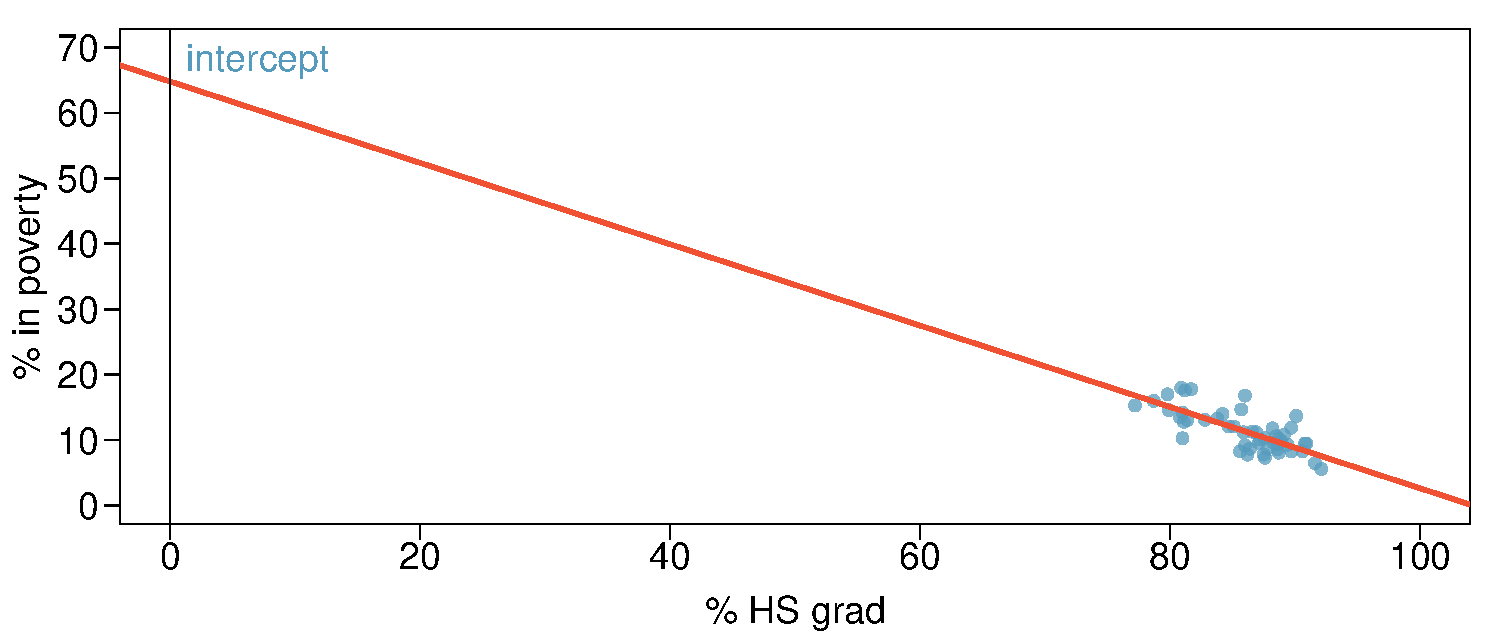
\includegraphics[width=\textwidth]{8-2_least_square_reg/figures/poverty/poverty_hsgrad_line_wide}
\end{center}

\end{frame}

%%%%%%%%%%%%%%%%%%%%%%%%%%%%%%%%%%

\begin{frame}
\frametitle{Examples of extrapolation}

\begin{center}
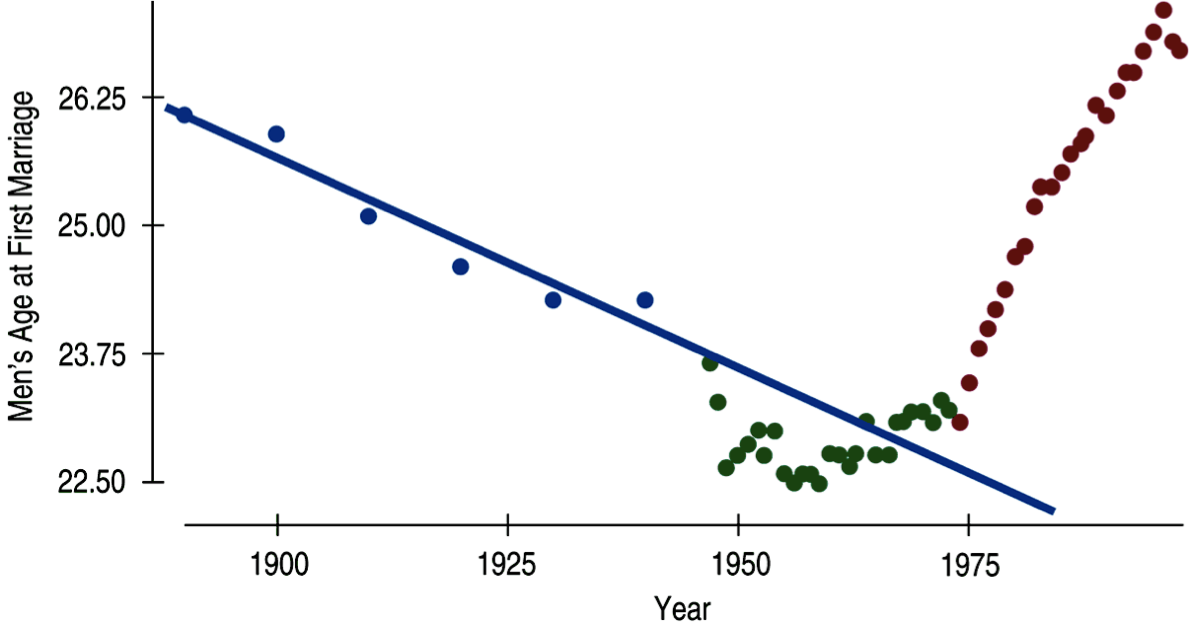
\includegraphics[width=\textwidth]{8-2_least_square_reg/figures/extrapolation}
\end{center}

\end{frame}

%%%%%%%%%%%%%%%%%%%%%%%%%%%%%%%%%%

\begin{frame}
\frametitle{Examples of extrapolation}

\begin{center}
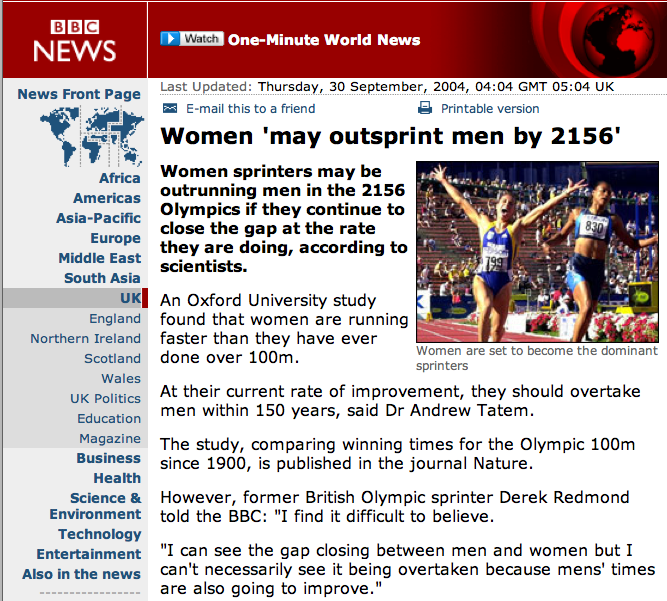
\includegraphics[width=0.7\textwidth]{8-2_least_square_reg/figures/womenOutsprintBBC}
\end{center}

\end{frame}

%%%%%%%%%%%%%%%%%%%%%%%%%%%%%%%%%%

\begin{frame}
\frametitle{Examples of extrapolation}

\begin{center}
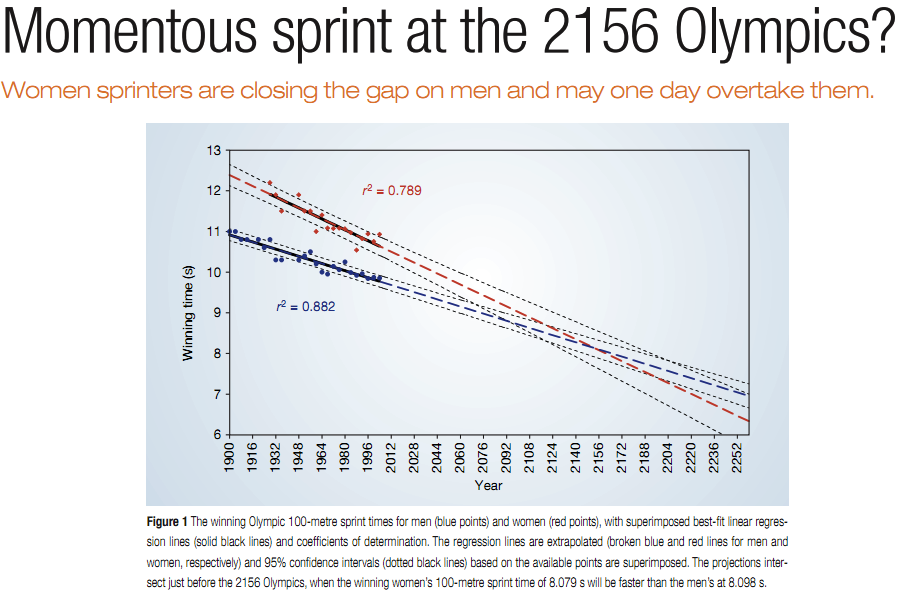
\includegraphics[width=\textwidth]{8-2_least_square_reg/figures/womenOutsprint}
\end{center}

\end{frame}

%%%%%%%%%%%%%%%%%%%%%%%%%%%%%%%%%%

\subsection{Conditions for the least squares line}

%%%%%%%%%%%%%%%%%%%%%%%%%%%%%%%%%%%

\begin{frame}
\frametitle{Conditions for the least squares line}

\begin{enumerate}

\item Linearity

\pause

\item Nearly normal residuals

\pause

\item Constant variability

\end{enumerate}

\end{frame}

%%%%%%%%%%%%%%%%%%%%%%%%%%%%%%%%%%

\begin{frame}
\frametitle{Conditions: (1) Linearity}

\begin{itemize}

\item The relationship between the explanatory and the response variable should be linear. 

\pause

\item Methods for fitting a model to non-linear relationships exist, but are beyond the scope of this class. If this topic is of interest, an \href{http://www.openintro.org/download.php?file=os2_extra_nonlinear_relationships&referrer=/stat/textbook.php}{Online Extra is available on openintro.org} covering new techniques.

\pause

\item Check using a scatterplot of the data, or a \hl{residuals plot}.

\end{itemize}

\begin{center}
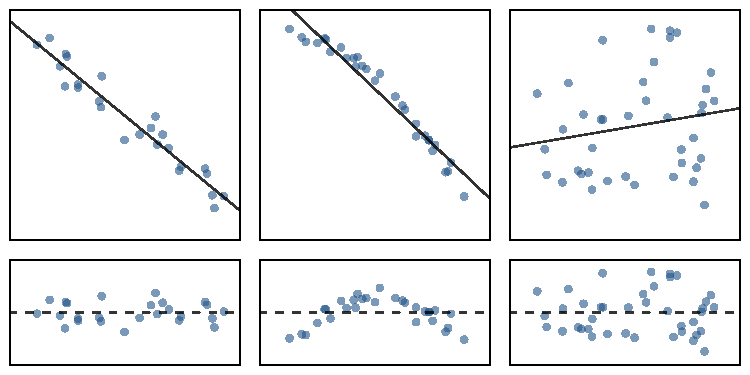
\includegraphics[width=0.7\textwidth]{8-2_least_square_reg/figures/sampleLinesAndResPlots/sampleLinesAndResPlots}
\end{center}

\end{frame}

%%%%%%%%%%%%%%%%%%%%%%%%%%%%%%%%%%

\begin{frame}
\frametitle{Anatomy of a residuals plot}

\twocol{0.5}{0.5}
{
\begin{center}
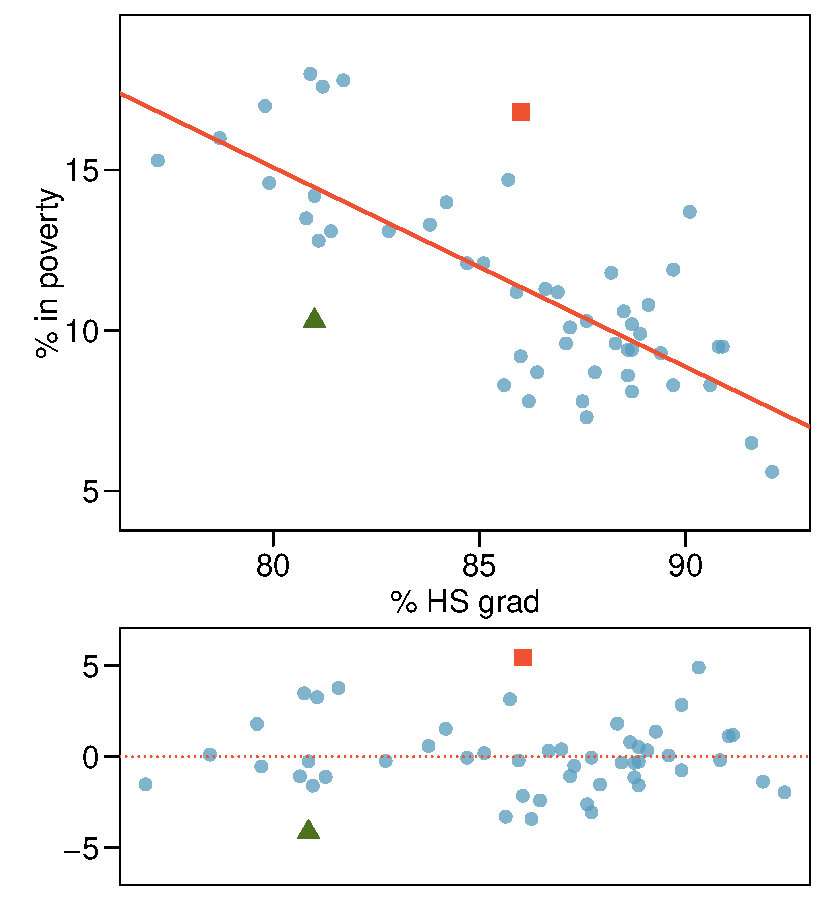
\includegraphics[width=\textwidth]{8-2_least_square_reg/figures/poverty/poverty_hsgrad_resplot}
\end{center}
}
{
\green{{\LARGE $\blacktriangle$}} \hl{RI:}
\begin{align*}
\%~HS~grad &= 81 \qquad \%~in~poverty = 10.3 \\
\widehat{\%~in~poverty} &= 64.68 - 0.62 * 81 = 14.46 \\
e &= \%~in~poverty - \widehat{\%~in~poverty} \\
&= 10.3 - 14.46 = \green{$-4.16$}
\end{align*}
$\:$
\pause
\textcolor{red}{{\Large $\blacksquare$}} \hl{DC:}
\begin{align*}
\%~HS~grad &= 86 \qquad \%~in~poverty = 16.8 \\
\widehat{\%~in~poverty} &= 64.68 - 0.62 * 86 = 11.36 \\
e &= \%~in~poverty - \widehat{\%~in~poverty} \\
&= 16.8 - 11.36 = \textcolor{red}{5.44}
\end{align*}
}

\end{frame}


%%%%%%%%%%%%%%%%%%%%%%%%%%%%%%%%%%

\begin{frame}
\frametitle{Conditions: (2) Nearly normal residuals}

\begin{itemize}

\item The residuals should be nearly normal.

\pause

\item This condition may not be satisfied when there are unusual observations that don't follow the trend of the rest of the data.

\pause

\item Check using a histogram or normal probability plot of residuals.

\end{itemize}

\begin{center}
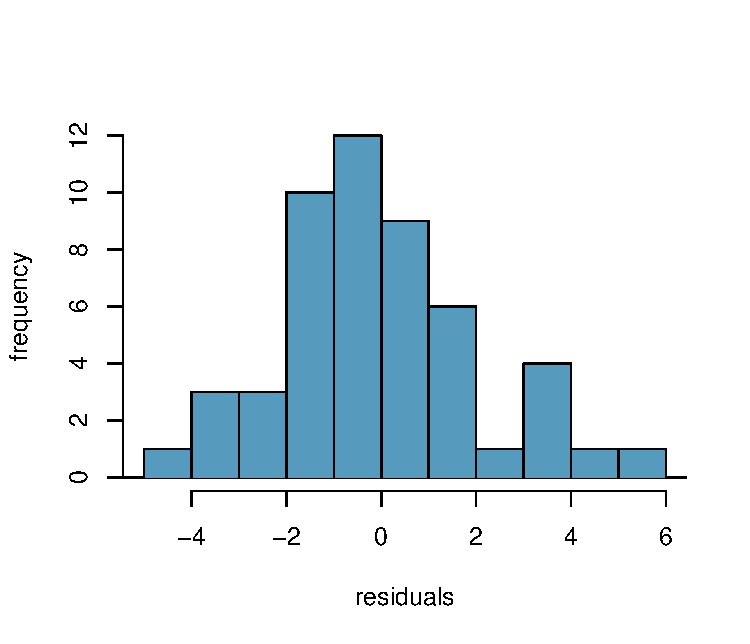
\includegraphics[width=\textwidth]{8-2_least_square_reg/figures/poverty/normal_res}
\end{center}

\end{frame}

%%%%%%%%%%%%%%%%%%%%%%%%%%%%%%%%%%

\begin{frame}
\frametitle{Conditions: (3) Constant variability}

\twocol{0.5}{0.5}
{
\begin{center}
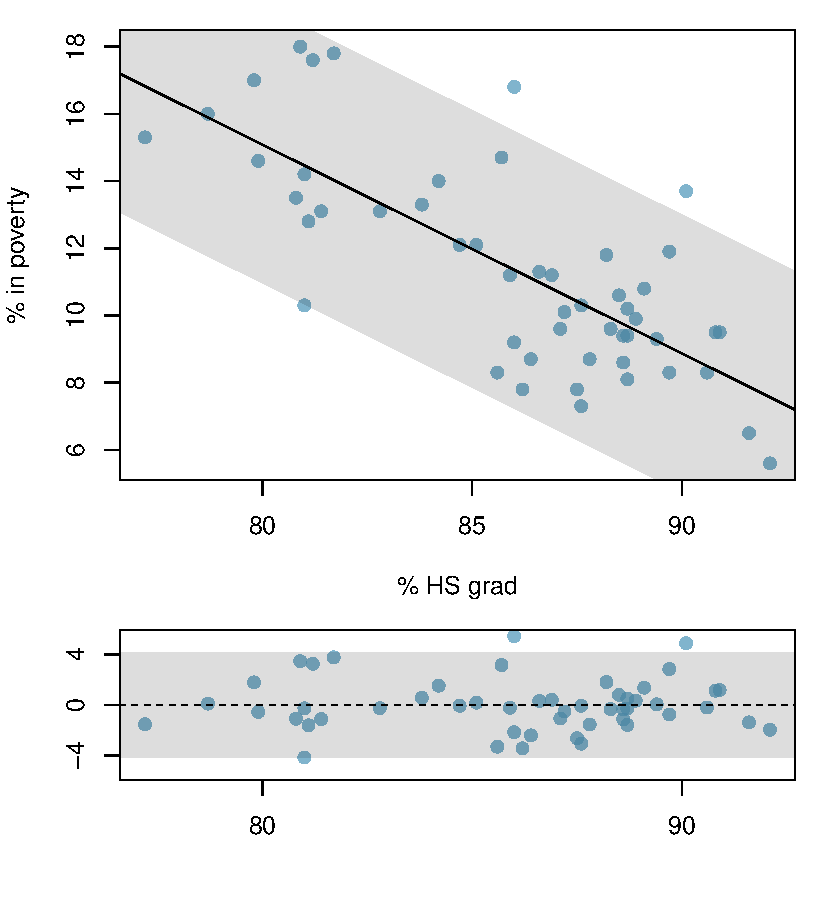
\includegraphics[width=\textwidth]{8-2_least_square_reg/figures/poverty/poverty_hsgrad_tube}
\end{center}
}
{
\begin{itemize}

\item The variability of points around the least squares line should be roughly constant.

\pause

\item This implies that the variability of residuals around the 0 line should be roughly constant as well.

\pause

\item Also called \hl{homoscedasticity}.

\pause

\item Check using a histogram or normal probability plot of residuals.

\end{itemize}
}


\end{frame}

%%%%%%%%%%%%%%%%%%%%%%%%%%%%%%%%%%

\begin{frame}
\frametitle{Checking conditions}

\twocol{0.5}{0.5}
{
\pq{What condition is this linear model obviously violating?}
\begin{enumerate}[(a)]
\item Constant variability
\solnMult{Linear relationship}
\item Normal residuals
\item No extreme outliers
\end{enumerate}
}
{
\begin{center}
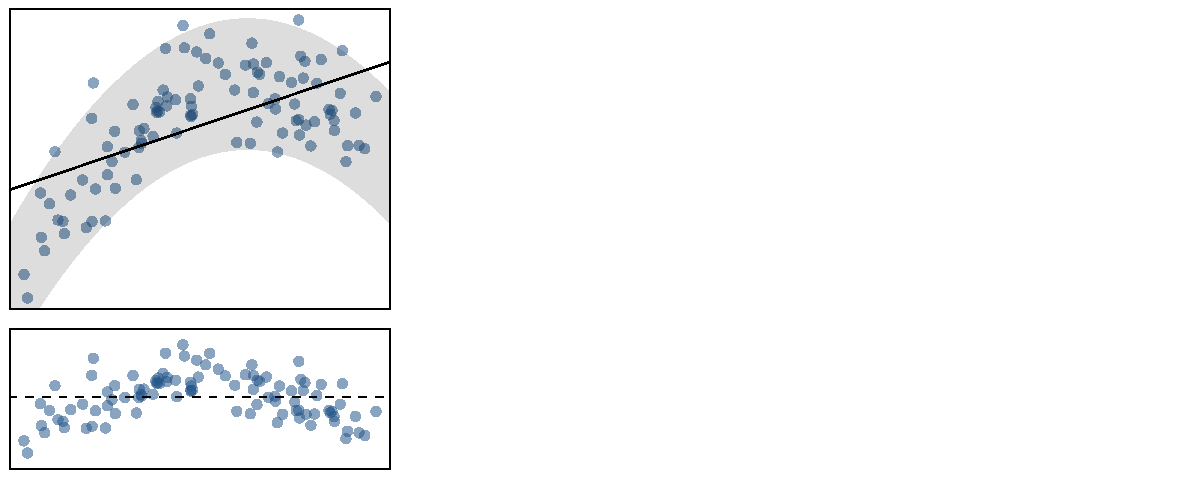
\includegraphics[width=\textwidth]{8-2_least_square_reg/figures/problems/nonlinear}
\end{center}
}

\end{frame}

%%%%%%%%%%%%%%%%%%%%%%%%%%%%%%%%%%

\begin{frame}
\frametitle{Checking conditions}

\twocol{0.5}{0.5}
{
\pq{What condition is this linear model obviously violating?}
\begin{enumerate}[(a)]
\solnMult{ Constant variability}
\item Linear relationship
\item Normal residuals
\item No extreme outliers
\end{enumerate}
}
{
\begin{center}
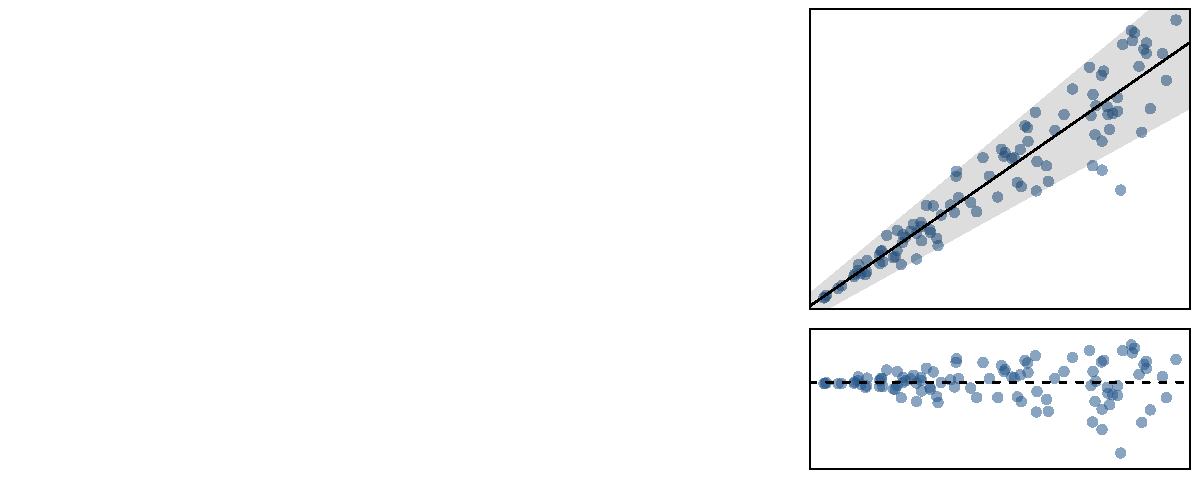
\includegraphics[width=\textwidth]{8-2_least_square_reg/figures/problems/heteroscedastic}
\end{center}
}

\end{frame}

%%%%%%%%%%%%%%%%%%%%%%%%%%%%%%%%%%

\subsection{$R^2$}

%%%%%%%%%%%%%%%%%%%%%%%%%%%%%%%%%%%

\begin{frame}
\frametitle{$R^2$}

\begin{itemize}

\item The strength of the fit of a linear model is most commonly evaluated using \mathhl{R^2}.

\pause

\item $R^2$ is calculated as the square of the correlation coefficient.

\pause

\item It tells us what percent of variability in the response variable is explained by the model.

\pause

\item The remainder of the variability is explained by variables not included in the model or by inherent randomness in the data.

\pause

\item For the model we've been working with, $R^2 = -0.62^2 = 0.38$.

\end{itemize}

\end{frame}

%%%%%%%%%%%%%%%%%%%%%%%%%%%%%%%%%%

\begin{frame}
\frametitle{Interpretation of $R^2$}

\pq{{\small Which of the below is the correct interpretation of $R = -0.62$, $R^2 = 0.38$?}}

\twocol{0.65}{0.35}{
\begin{enumerate}[(a)]

\item 38\% of the variability in the \% of HG graduates among the 51 states is explained by the model.

\solnMult{ 38\% of the variability in the \% of residents living in poverty among the 51 states is explained by the model.}

\item 38\% of the time \% HS graduates predict \% living in poverty correctly.

\item 62\% of the variability in the \% of residents living in poverty among the 51 states is explained by the model.

\end{enumerate}
}{
\begin{center}
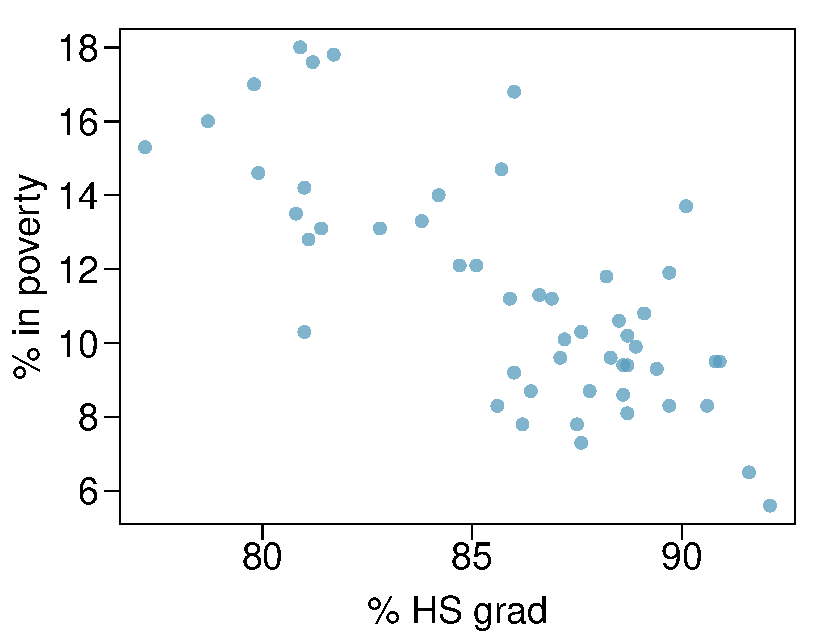
\includegraphics[width=\textwidth]{8-2_least_square_reg/figures/poverty/poverty_hsgrad}
\end{center}
}

\end{frame}

%%%%%%%%%%%%%%%%%%%%%%%%%%%%%%%%%%

\subsection{Categorical explanatory variables}

%%%%%%%%%%%%%%%%%%%%%%%%%%%%%%%%%%%

\begin{frame}
\frametitle{Poverty vs. region (east, west)}


\[ \widehat{poverty} = 11.17 + 0.38 \times west \]

\begin{itemize}

\item Explanatory variable: region, \hl{reference level:} east

\item \hl{Intercept:} The estimated average poverty percentage in eastern states is 11.17\%
\pause
\begin{itemize}
\item This is the value we get if we plug in \orange{0} for the explanatory variable
\end{itemize}

\pause

\item \hl{Slope:} The estimated average poverty percentage in western states is 0.38\% higher than eastern states.
\pause
\begin{itemize}
\item Then, the estimated average poverty percentage in western states is 11.17 + 0.38 =  11.55\%.
\pause
\item This is the value we get if we plug in \orange{1} for the explanatory variable
\end{itemize}

\end{itemize}

\end{frame}

%%%%%%%%%%%%%%%%%%%%%%%%%%%%%%%%%%

\begin{frame}
\frametitle{Poverty vs. region (northeast, midwest, west, south)}

\pq{Which region (northeast, midwest, west, or south) is the reference level?}

{\small
\begin{center}
\begin{tabular}{rrrrr}
  \hline
 & Estimate & Std. Error & t value & Pr($>$$|$t$|$) \\ 
  \hline
(Intercept) & 9.50 & 0.87 & 10.94 & 0.00 \\ 
region4midwest & 0.03 & 1.15 & 0.02 & 0.98 \\ 
region4west & 1.79 & 1.13 & 1.59 & 0.12 \\ 
region4south & 4.16 & 1.07 & 3.87 & 0.00 \\ 
   \hline
\end{tabular}
\end{center}
}

\begin{enumerate}[(a)]
\solnMult{northeast}
\item midwest
\item west
\item south
\item cannot tell
\end{enumerate}

\end{frame}

%%%%%%%%%%%%%%%%%%%%%%%%%%%%%%%%%%%

\begin{frame}
\frametitle{Poverty vs. region (northeast, midwest, west, south)}

\pq{Which region (northeast, midwest, west, or south) has the lowest poverty percentage?}

{\small
\begin{center}
\begin{tabular}{rrrrr}
  \hline
 & Estimate & Std. Error & t value & Pr($>$$|$t$|$) \\ 
  \hline
(Intercept) & 9.50 & 0.87 & 10.94 & 0.00 \\ 
region4midwest & 0.03 & 1.15 & 0.02 & 0.98 \\ 
region4west & 1.79 & 1.13 & 1.59 & 0.12 \\ 
region4south & 4.16 & 1.07 & 3.87 & 0.00 \\ 
   \hline
\end{tabular}
\end{center}
}

\begin{enumerate}[(a)]
\solnMult{northeast}
\item midwest
\item west
\item south
\item cannot tell
\end{enumerate}

\end{frame}
